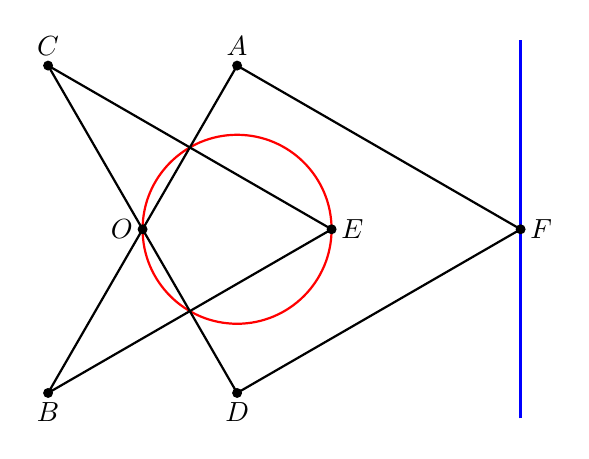
\begin{tikzpicture}[scale=1.2]

  % Foints on/around circle
  \def\len{2}
  \coordinate (A) at ({\len*cos(60)},{\len*sin(60)});
  \coordinate (C) at ({\len*-cos(60)},{\len*sin(60)});
  \coordinate (B) at ({\len*-cos(60)},{\len*-sin(60)});
  \coordinate (D) at ({\len*cos(60)},{\len*-sin(60)});

  % Circle 
  \def\r{1}
  \draw[red, thick] (\r,0) circle (\r);
  
  % Vertical line
  \coordinate (O) at (0,0);
  \coordinate (E) at ({2*\r},0);
  \coordinate (F) at ({2*\r+2*\len*cos(60)},0);
  \draw[blue, thick] ({2*\r+2*\len*cos(60)},-2) -- ({2*\r+2*\len*cos(60)},2);

  % Connections
  \draw[thick] (A) -- (O) -- (B) -- (E) -- (C);
  \draw[thick] (C) -- (D) -- (F) -- (A);

  % Mark points
  \fill (A) circle (1.5pt);
  \fill (B) circle (1.5pt);
  \fill (C) circle (1.5pt);
  \fill (D) circle (1.5pt);
  \fill (F) circle (1.5pt);
  \fill (E) circle (1.5pt);
  \fill (O) circle (1.5pt);

  % Labels
  \node[left] at (O) {$O$};
  \node[right] at (F) {$F$};
  \node[right] at (E) {$E$};
  \node[above] at (A) {$A$};
  \node[below] at (B) {$B$};
  \node[above] at (C) {$C$};
  \node[below] at (D) {$D$};

\end{tikzpicture}
